\documentclass[aspectratio=169, dvipdfmx, 11pt]{beamer}
\usepackage{here, amsmath, latexsym, amssymb, bm, ascmac, mathtools, multicol, tcolorbox, subfig}
\usepackage[scale=2]{ccicons}
\usepackage[sortcites,style=numeric,backend=biber]{biblatex}
\addbibresource{main.bib}

% \usepackage{enumitem}

\usetheme{metropolis} % Use metropolis theme
\setbeamercolor{background canvas}{bg=white}
\setbeamercolor{block title}{bg=white}

\DeclareFontFamily{U}{MnSymbolD}{}
\DeclareFontShape{U}{MnSymbolD}{m}{n}{
    <-6>  MnSymbolD5
   <6-7>  MnSymbolD6
   <7-8>  MnSymbolD7
   <8-9>  MnSymbolD8
   <9-10> MnSymbolD9
  <10-12> MnSymbolD10
  <12->   MnSymbolD12}{}
\DeclareFontShape{U}{MnSymbolD}{b}{n}{
    <-6>  MnSymbolD-Bold5
   <6-7>  MnSymbolD-Bold6
   <7-8>  MnSymbolD-Bold7
   <8-9>  MnSymbolD-Bold8
   <9-10> MnSymbolD-Bold9
  <10-12> MnSymbolD-Bold10
  <12->   MnSymbolD-Bold12}{}
\DeclareSymbolFont{MnSyD}{U}{MnSymbolD}{m}{n}
\SetSymbolFont{MnSyD}{bold}{U}{MnSymbolD}{b}{n}

\DeclareMathSymbol\preccurlyeq{\mathrel}{MnSyD}{"6C}
\DeclareMathSymbol\npreccurlyeq{\mathrel}{MnSyD}{"E4}

% Mathematical Sets
\newcommand{\NaturalNumberSet}{\mathbb{N}}
\newcommand{\RealNumberSet}{\mathbb{R}}
\newcommand{\NDemenstionalRealEuclideanSpace}{\mathbb{R}^n}
\newcommand{\NDemenstionalRealSymmetricMatrixSpace}{\mathbb{S}^n}

% Symbols of prefix
\newcommand{\Closure}[1]{\text{\rm cl\:${#1}$}} % cl
\newcommand{\Interior}[1]{\text{\rm int\:${#1}$}} % int
\newcommand{\Domain}[1]{\text{\rm dom\:${#1}$}} % dom
\newcommand{\Epigraph}[1]{\text{\rm epi\:${#1}$}} % epi
\newcommand{\Trace}[1]{\text{\rm tr$({#1})$}} % tr
\newcommand{\InnerProduct}[2]{\left\langle {#1},{#2}\right\rangle} % <x,y>
\newcommand{\OrderingLevelSets}[3]{\text{\rm lev\:$({#1}, {#2}, {#3})$}} % lev
\newcommand{\Nbd}[2]{\mbox{$\mathcal{N}_{#1}({#2})$}}
\newcommand{\Norm}[1]{\left\lVert {#1} \right\rVert} % ||x||

% Extended real valued function e.g. f: X -> Rv{+∞}
% #1: function symbol
% #2: domain of function
\newcommand{\ExtendedRealValuedFunction}[2]{{#1}: {#2} \to \RealNumberSet \cup \{+\infty\}}

% Conjugate function e.g. f*
% #1: function symbol
\newcommand{\ConjugateFunction}[1]{{#1}^*}

% (Useful) Texts
\newcommand{\SuchThat}{\:\text{s.t.}\:}

% Set form e.g. {x | ...}
% #1: element
% #2: conditions
\newcommand{\SetForm}[2]{
  \{{#1}\:|\:{#2}\}
}

\title{スカラー化関数による集合値関数のミニマックス定理の一般化とその応用}
\subtitle{Set-Valued Fan-Takahashi Inequalities Via Scalarization}
\author[Ryota Iwamoto]{Ryota Iwamoto* and Tamaki Tanaka}
\institute[Niigata Univ]{Niigata Univ}
\date{27th, October, 2024}
\titlegraphic{
  \vspace{5cm}
  \hspace{11cm}
  \includegraphics[keepaspectratio, scale=0.20]{figures/niigata_university_logo.png}
  }

\begin{document}
\maketitle

\begin{frame}{Contents}
  \tableofcontents
\end{frame}

% 1. Introduction
% ----------------------------------------------------------------
\section{Introduction}

% scalar optimization problem
\begin{frame}{What is set optimization problem?}
  \begin{itemize}
    \item To find a footballer from a set of football players who
          has the least (or most) number of goals is
          the \textcolor{red}{scalar~optimization~problem}
          where the objective function provides the number
          of goals of a player.
  \end{itemize}
  \centering
  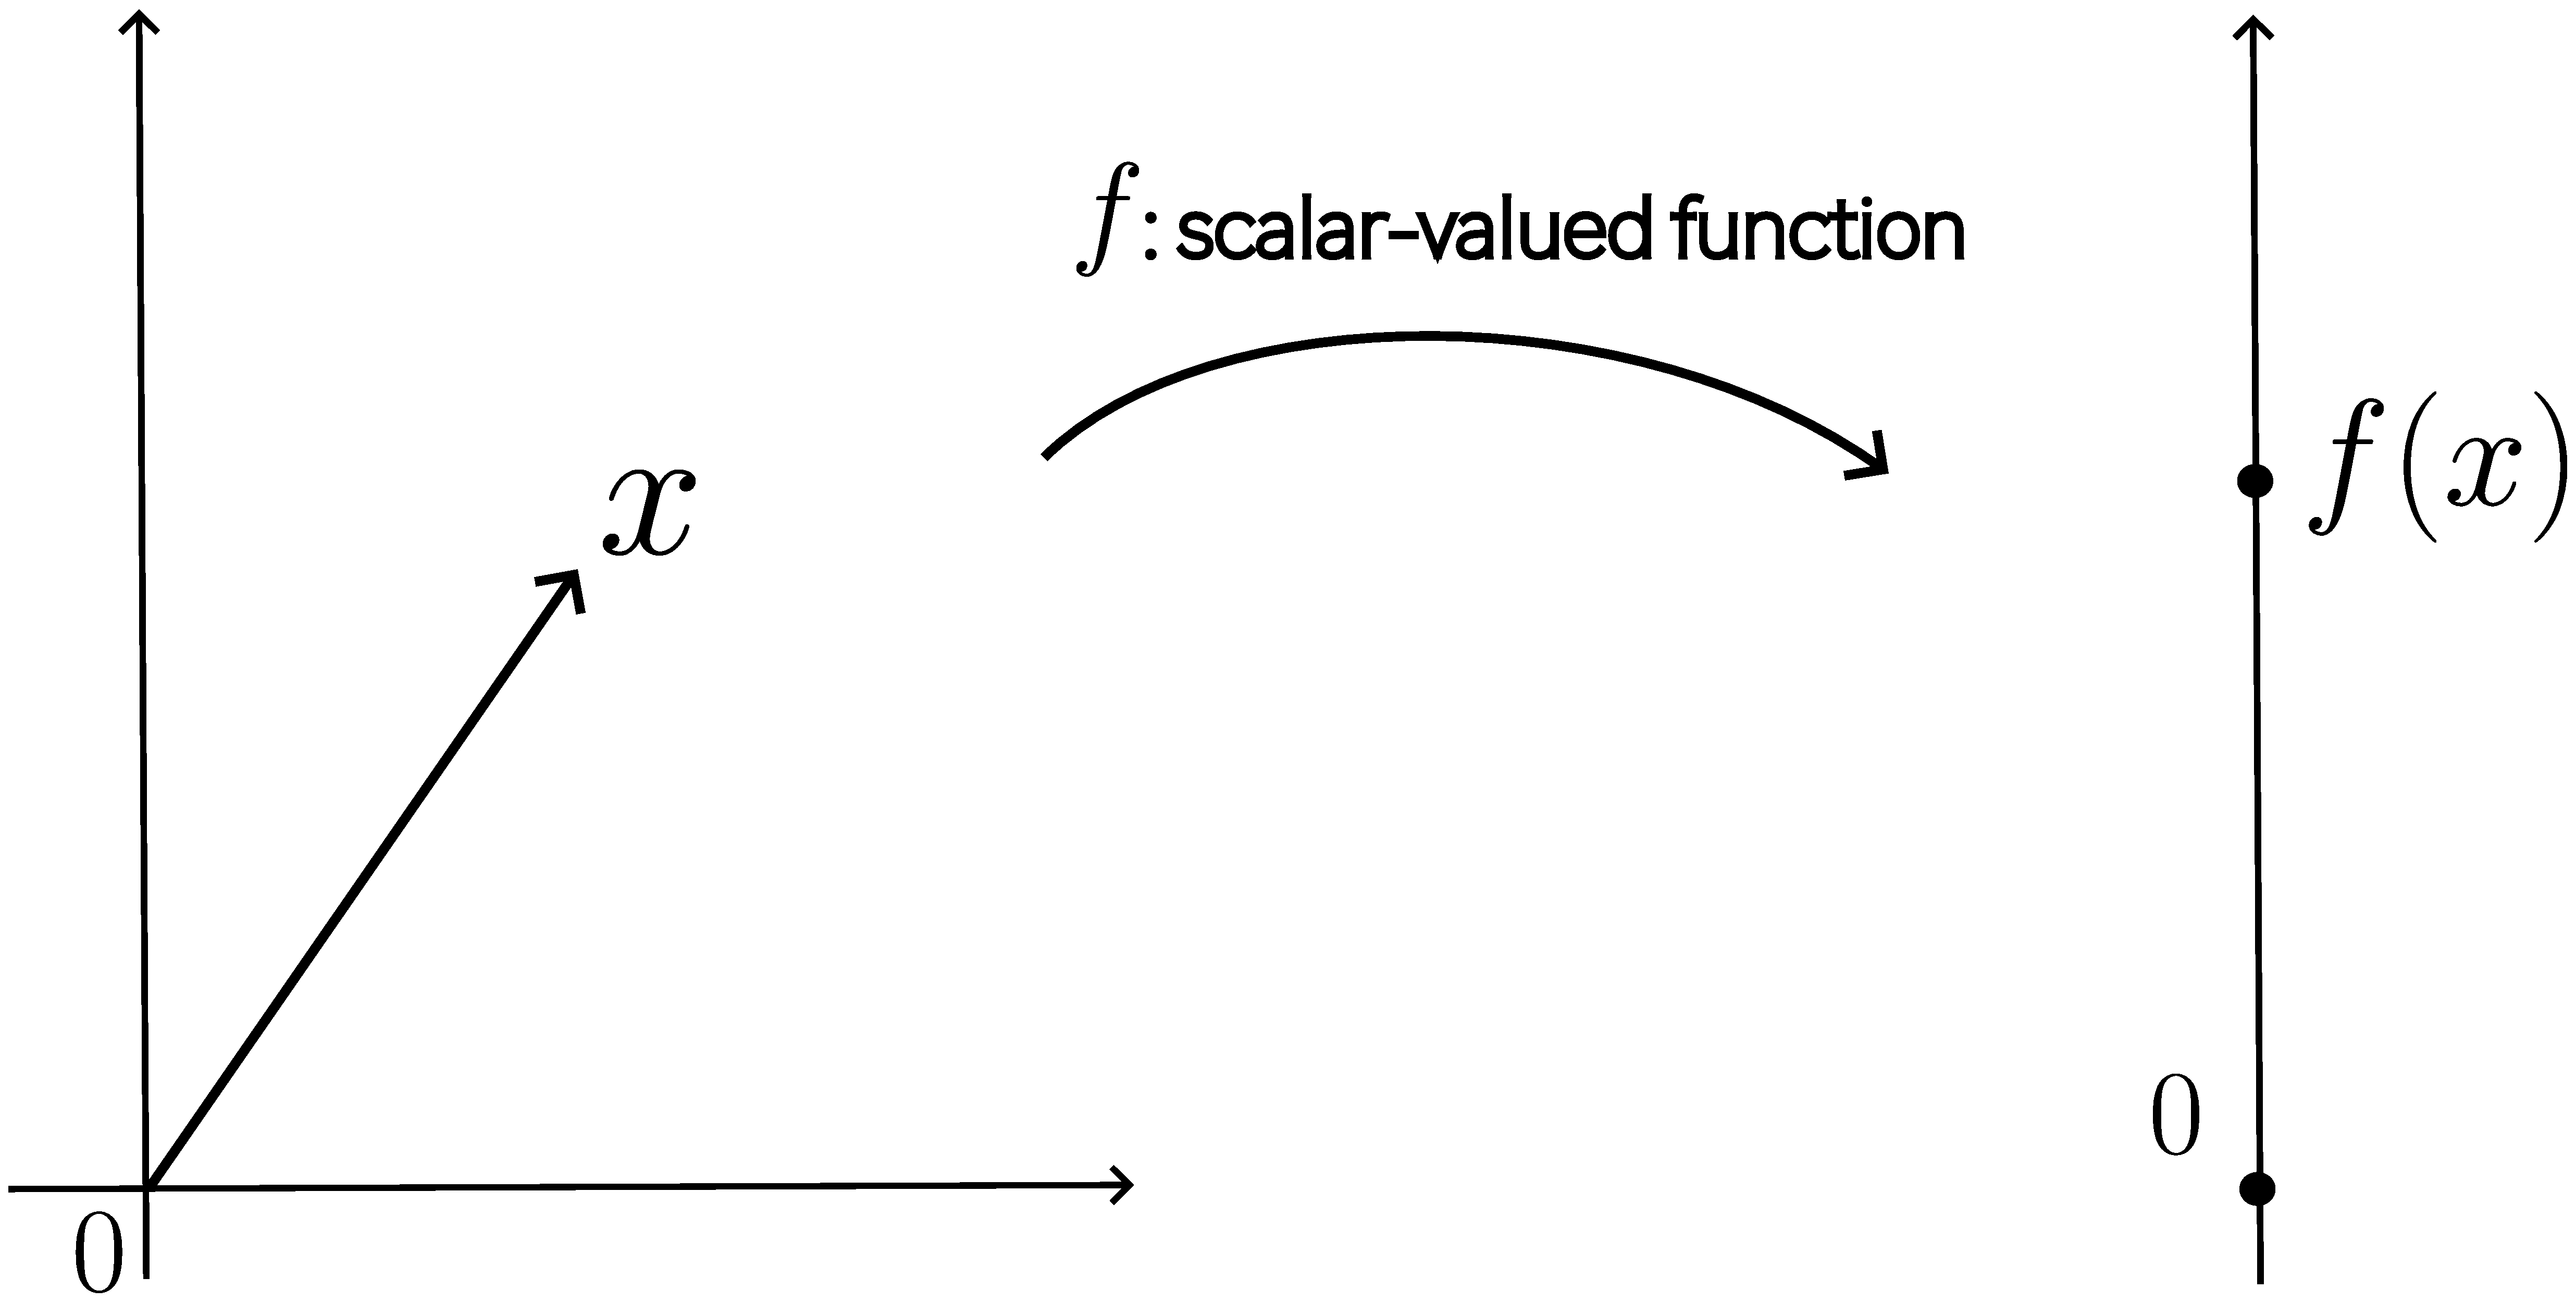
\includegraphics[keepaspectratio, scale=0.08]{figures/eps/scalar_opt.eps}
  \renewcommand{\thefootnote}{\fnsymbol{footnote}}%
  \footnote[0]{Reference: \url{https://agates.mimuw.edu.pl/images/nonworkshop_talks/Sharma_slides.pdf}}
\end{frame}

% vector optimization problem
\begin{frame}{What is set optimization problem?}
  \begin{itemize}
    \item To find the football player from a set of footballers in such a way that he/she
          is having several qualities, namely, ability, speed, power, and so on,
          is a \textcolor{red}{vector~optimization~problem}. The value of the objective function can be
          considered as vector whose coordinates consist of one's ability, speed, power, and so on.
  \end{itemize}
  \centering
  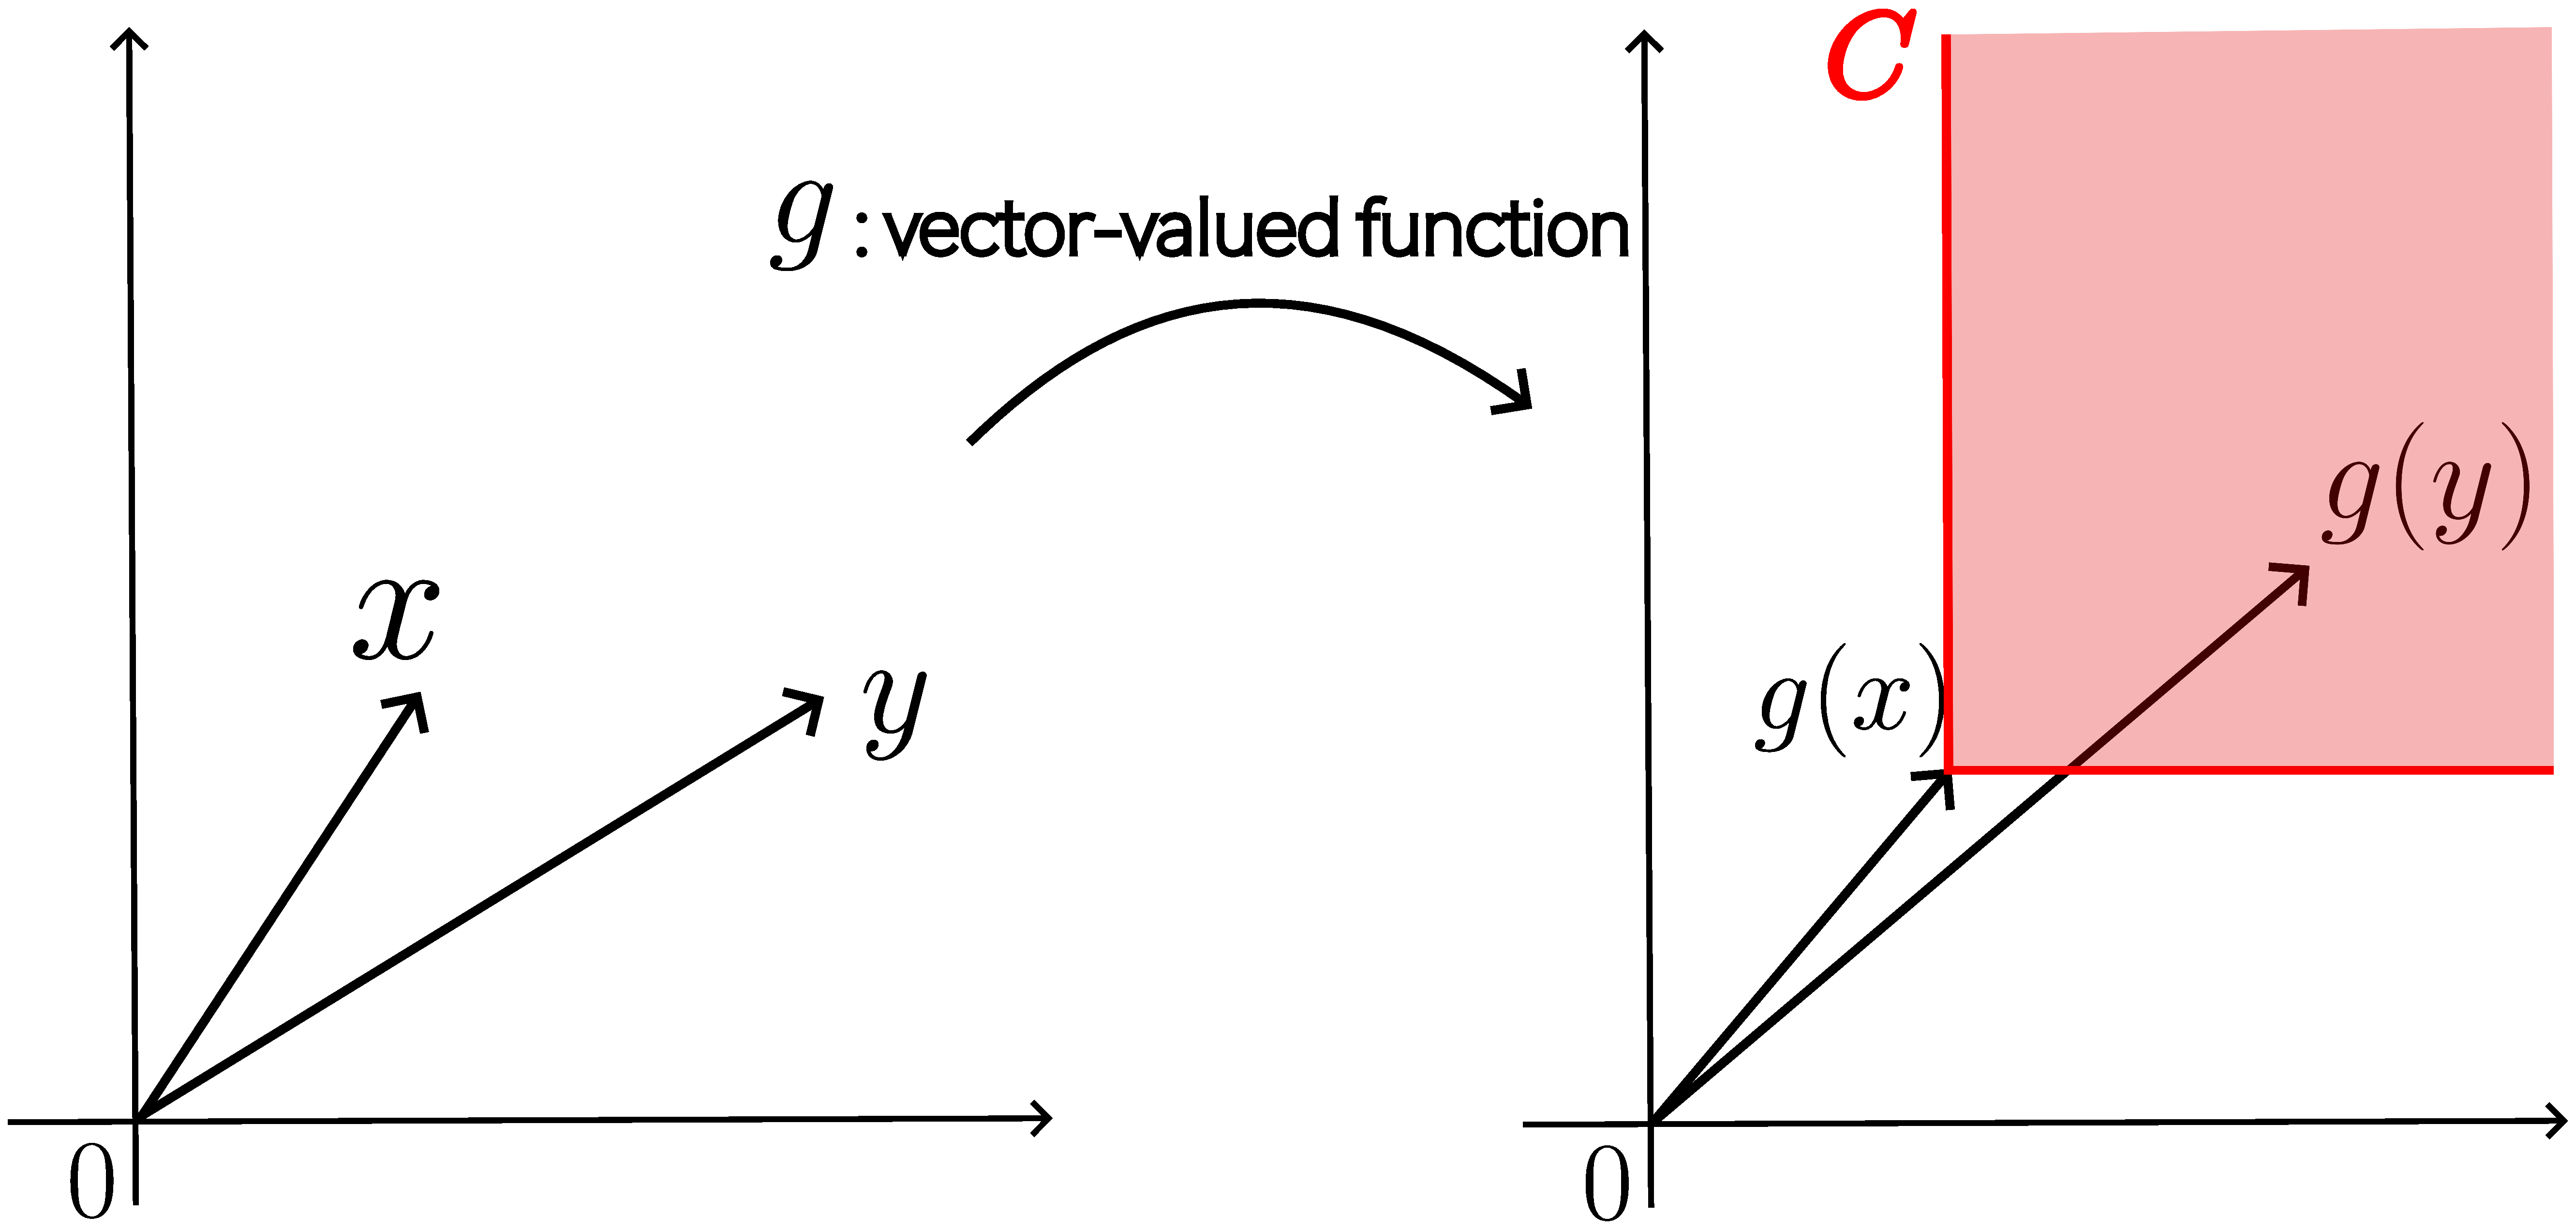
\includegraphics[keepaspectratio, scale=0.07]{figures/eps/vector_opt.eps}
  \renewcommand{\thefootnote}{\fnsymbol{footnote}}%
  \footnote[0]{Reference: \url{https://agates.mimuw.edu.pl/images/nonworkshop_talks/Sharma_slides.pdf}}
\end{frame}

% set optimization problem
\begin{frame}{What is set optimization problem?}
  \begin{itemize}
    \item Consider the objective function whose values are teams and assume
          that a team is a set of football players and each player is
          regarded as a vector whose coordinates consist of one's ability,
          speed, power, stamina, skill, popularity and so on. Then one
          can formulate the problem of choosing a good team for a football league in the form
          of \textcolor{red}{set~optimization~problem} with the set-valued objective function.
  \end{itemize}
  \centering
  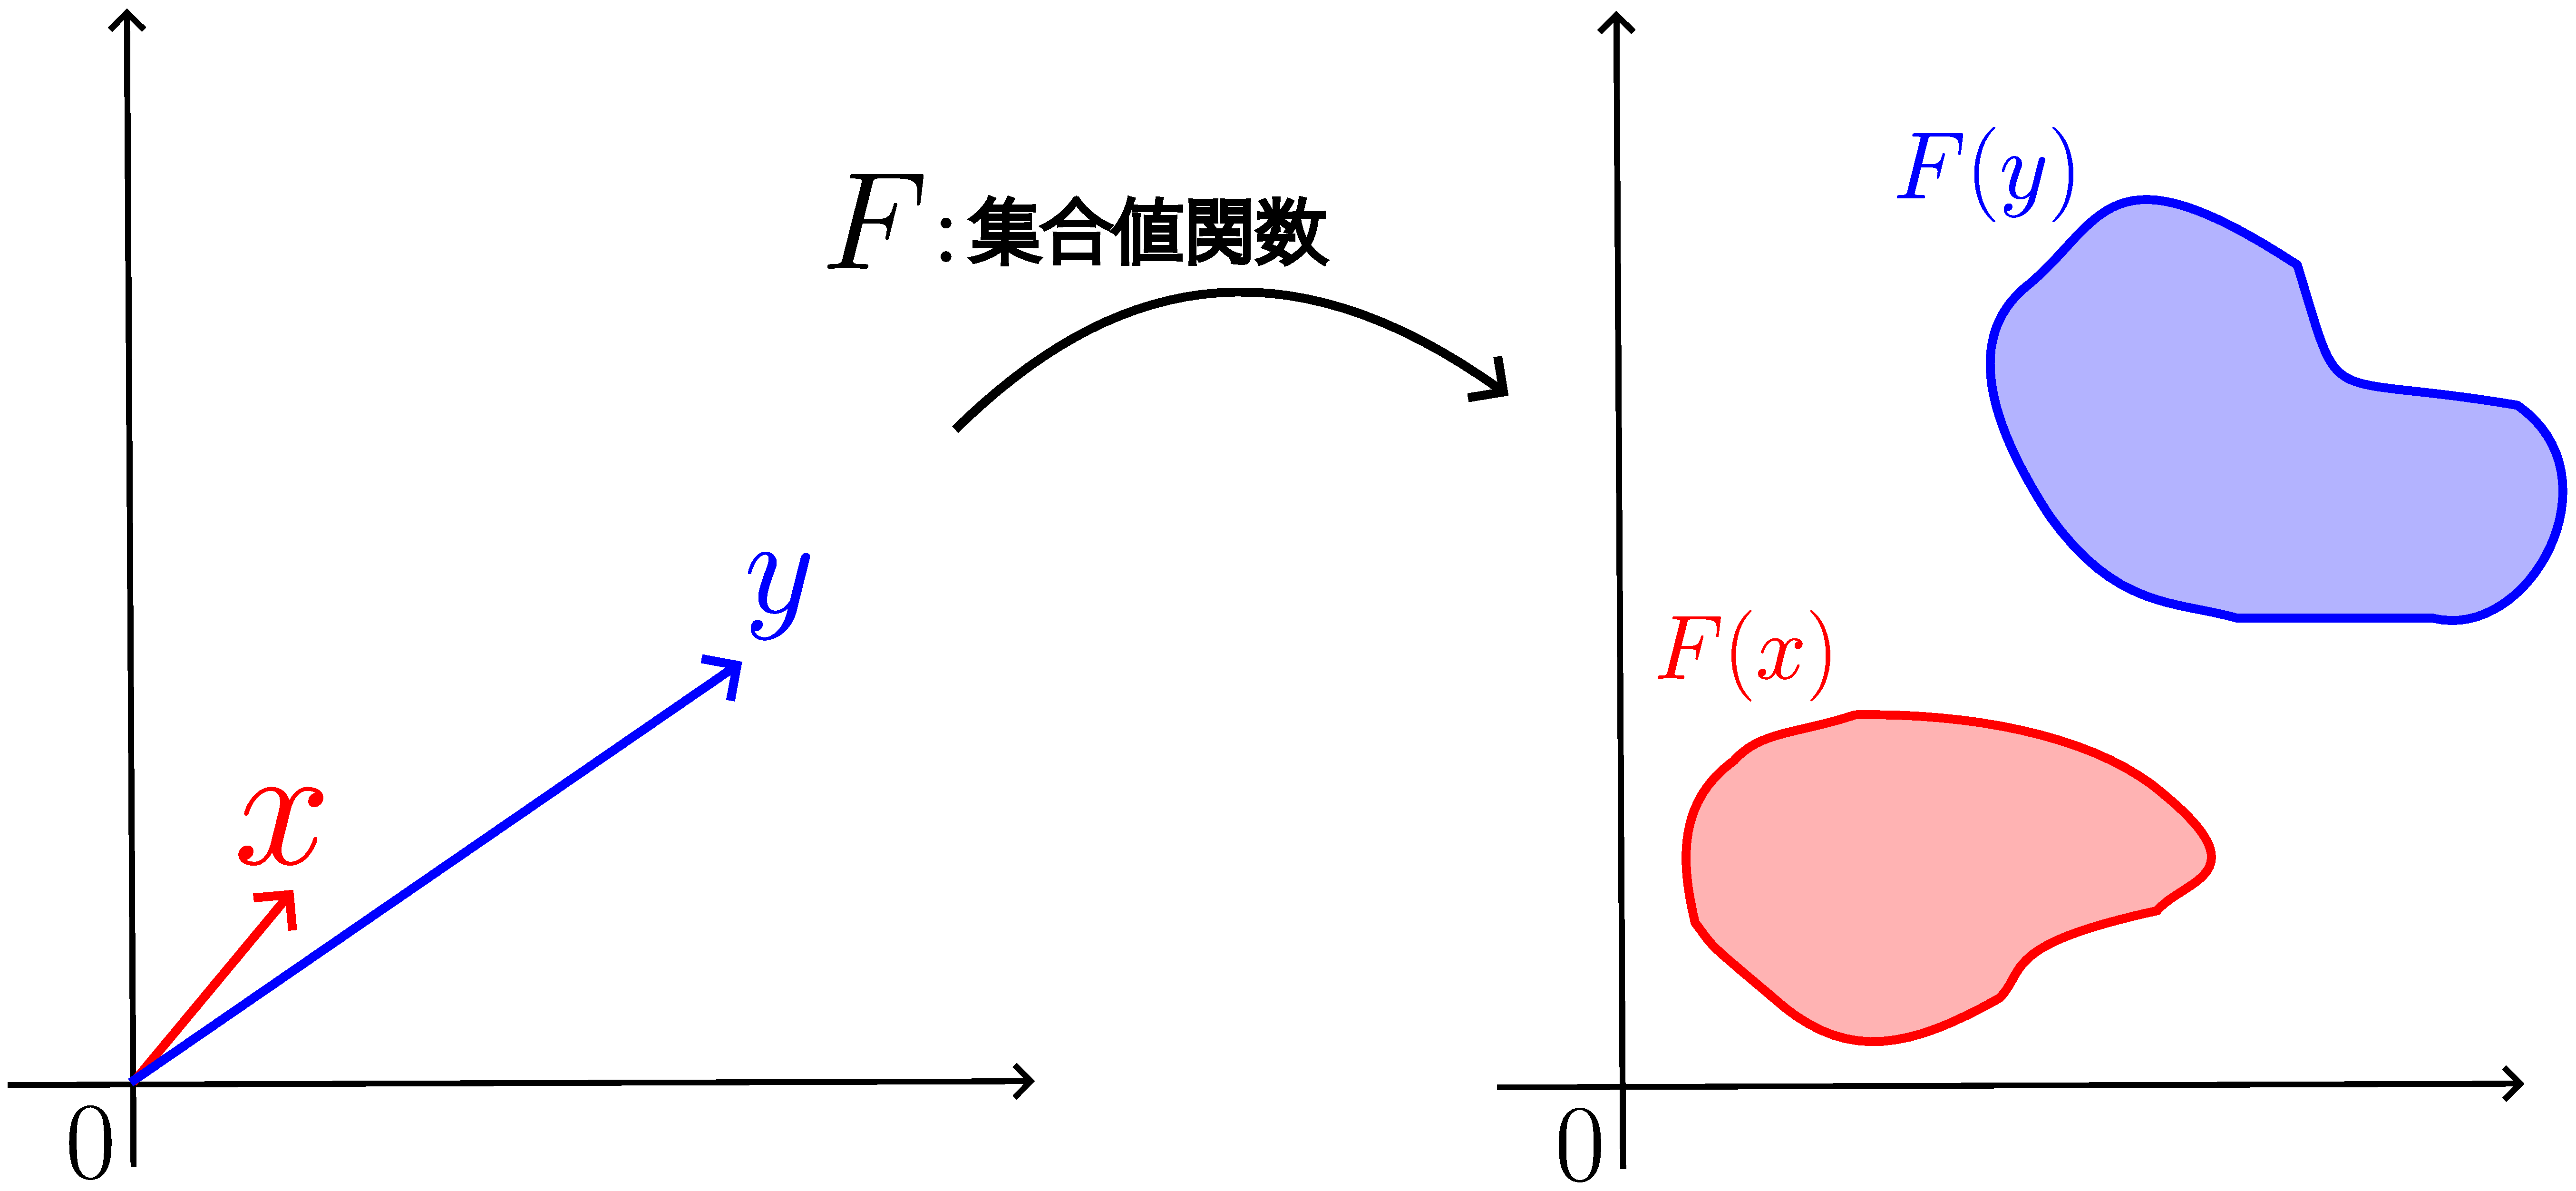
\includegraphics[keepaspectratio, scale=0.07]{figures/eps/set_opt.eps}
  \renewcommand{\thefootnote}{\fnsymbol{footnote}}%
  \footnote[0]{Reference: \url{https://agates.mimuw.edu.pl/images/nonworkshop_talks/Sharma_slides.pdf}}
\end{frame}

% 2. Background
% ----------------------------------------------------------------
\section{Background}

\begin{frame}{Background}
  - Georgiev and Tanaka \cite{MR1807037} extended the minimax inequality to the form of set-valued maps.
  % P. G. Georgiev と T. Tanaka によって集合値への minimax 不等式の拡張が進められた。

  - Kuwano, Tanaka, and Yamada \cite{MR2778674} constructed the result of four types set-valued minimax inequalities
  with set relations.
  % I. Kuwano と T. Tanaka, S. Yamada によって set-relations の比較にに対してスカラー関数を対応させたものの minimax 不等式の拡張が進められた。

  - \textbf{Our goal is to generalize the result of four types set-valued minimax inequalities which is independent on the specific set-relations and scalarization functions.}
  % set-relations の比較に依存しない形、またスカラー化関数がその比較に依存しない形を目指す。
\end{frame}

\begin{frame}{Background}
  \begin{block}{Theorem (Takahashi \cite{MR399979} in 1976)} % 高橋先生の論文を引用する形に変更
    Let $X$ be a nonempty compact convex subset of a Hausdorff topological vector space and $f \colon X \times X \to \RealNumberSet$. If $f$ satisfies
    the following conditions:
    \begin{enumerate}
      \item for each fixed $y \in X$, $f(\cdot,y)$ is lower semicontinuous,
      \item for each fixed $x \in X$, $f(x,\cdot)$ is quasi concave,
      \item $f(x,x) \leq 0$ for all $x \in X$,
    \end{enumerate}
    then there exists $\bar{x} \in X$ such that $f(\bar{x},y) \leq 0$ for all $y \in X$.
  \end{block}
\end{frame}

\begin{frame}{Background}
  \begin{block}{Theorem \cite{MR2778674}}
    Let $X$ be a nonempty compact convex subset of a Hausdorff topological vector space,
    $Y$ a real topological vector space, $C$ a proper closed convex cone in $Y$ with $\Interior{C} \ne \emptyset$
    and $F\colon X \times X \to \mathcal{P}(Y) \backslash \{\emptyset\}$. If $F$ satisfies the following conditions:
    \begin{enumerate}
      \item $F$ is $C$-proper and $C$-closed on $X \times X$,
      \item for each fixed $y \in X$, $F(\cdot,y)$ is $C$-upper continuous,
      \item for each fixed $x \in X$, $f(x, \cdot)$ is type (3L) properly $C$-quasi concave,
      \item for all $x \in X$, $F(x,x) \preccurlyeq_{C}^{(3L)} \{\theta_{Y}\}$,
    \end{enumerate}
    then there exists $\bar{x} \in X$ such that $F(\bar{x},y) \preccurlyeq_{C}^{(3L)} \{\theta_{Y}\}$ for all $y \in X$.
  \end{block}
\end{frame}

% 3. Preliminaries
% ----------------------------------------------------------------
\section{Preliminaries}

\begin{frame}{Preliminaries}
  Let $X$ be a topological space, $Y$ a real topological vector space, and $\theta_Y$ be a zero vector in $Y$.
  Define that $\mathcal{P}(Y)$ is the set of all nonempty subsets of $Y$.
  The sets of neighborhoods of $x \in X$ and $y \in Y$ is denoted by $\mathcal{N}_X (x)$ and $\mathcal{N}_Y (y)$, respectively.

  \begin{block}{Definition}
    For $A,B \in \mathcal{P}(Y) \backslash \{\emptyset\}$, we define two binary relations on $\mathcal{P}(Y)$:
    \begin{equation}
      A \preccurlyeq_1 B \overset{\text{def}}{\Longleftrightarrow} A \cap B \ne \emptyset \quad \text{and} \quad A \preccurlyeq_2 B \overset{\text{def}}{\Longleftrightarrow} B \subset A. \notag
    \end{equation}
  \end{block}

  \begin{block}{Definition (set-relations)}
    For $A,B \in \mathcal{P}(Y) \backslash \{\emptyset\}$ and a convex cone $C$, we write
    \begin{equation}
      A \preccurlyeq_{C}^{(3L)} B \overset{\text{def}}{\Longleftrightarrow} B \subset A + C
      \quad \text{and} \quad A \preccurlyeq_{C}^{(3U)} B \overset{\text{def}}{\Longleftrightarrow} A \subset B -C. \notag
    \end{equation}
  \end{block}
\end{frame}

\begin{frame}{Preliminaries (Lower Semicontinuity)}
  \begin{block}{Definition}
    Let $f:Y\rightarrow \RealNumberSet \cup \{ \pm \infty\}$ and $y_{0}\in{Y}$.
    We say that $f$ is
    lower semicontinuous (l.s.c.\ shortly) at $y_{0}$ if
    \begin{equation}
      \forall r < f \left( y_{0} \right),
      \exists V \in \Nbd{Y}{y_{0}} \:\SuchThat\: r < f \left( y \right),\: \forall y \in V; \notag
    \end{equation}
  \end{block}

  \begin{block}{Definition \cite{500001551932}}
    Let $F \colon X \to \mathcal{P}(Y)$, $x_0 \in X$, $\preccurlyeq$ a binary relation on $\mathcal{P}(Y)$
    and $C \subset Y$ a convex cone. We say that $F$ is $(\preccurlyeq, C)$-continuous at $x_0$ if
    \begin{equation}
      \forall W \subset Y, W\:\text{open},W \preccurlyeq F(x_0), \exists V \in \mathcal{N}_{X}(x_0) \:\SuchThat\: W + C \preccurlyeq F(x), \forall x \in V. \notag
    \end{equation}
  \end{block}

  \begin{alertblock}{Remark}
    As special cases, $(\preccurlyeq_1, C)$-continuity and $(\preccurlyeq_2, C)$-continuity coincide with “C-lower
    continuity” and “C-upper continuity” for set-valued maps, respectively.
  \end{alertblock}
\end{frame}

\begin{frame}{Preliminaries (Lower Semicontinuity)}
  \begin{block}{Definition \cite{500001551932}}
    Let $\varphi \colon \mathcal{P}(Y) \to \RealNumberSet \cup \{\pm \infty\}$, $A_0 \in \mathcal{P}(Y)$,
    $\preccurlyeq$ a binary relation on $\mathcal{P}(Y)$, and $C$ a convex cone in $Y$ with $C \ne Y$. Then,
    we say that $\varphi$ is $(\preccurlyeq, C)$-lower semicontinuous at $A_0$ if
    \begin{equation}
      \forall r < \varphi (A_0), \exists W \in \mathcal{P}(Y), W\:\text{open}, \SuchThat W \preccurlyeq A_0 \:\text{and}\:
      r > \varphi (A), \forall A \in U(W + C, \preccurlyeq); \notag
    \end{equation}
    where $U(V,\preccurlyeq) \coloneqq \SetForm{A \in \mathcal{P}(Y)}{V \preccurlyeq A}$.
  \end{block}

  \begin{block}{Theorem \cite{500001551932}}
    Let $F \colon X \to \mathcal{P}(Y)$, $\varphi \colon \mathcal{P}(Y) \to \RealNumberSet \cup \{\pm \infty\}$, $x_0 \in X$,
    $\preccurlyeq$ a binary relation on $\mathcal{P}(Y)$, and $C$ a convex cone. If $F$ is $(\preccurlyeq, C)$-continuous at $x_0$
    and $\varphi$ is $(\preccurlyeq, C)$-lower semicontinuous at $F(x_0)$, then $(\varphi \circ F)$ is lower semicontinuous at $x_0$.
  \end{block}
\end{frame}

\begin{frame}{Preliminaries (Convexity)}
  \begin{block}{Definition \cite{MR3458699}}
    Let $\mathcal{A} \subset \mathcal{P}(Y) \backslash \{\emptyset\}$. $\mathcal{A}$ is said to be convex if for each $A_1, A_2 \in \mathcal{A}$ and $\lambda \in (0,1)$,
    \begin{equation}
      \lambda A_1 + (1-\lambda) A_2 \in \mathcal{A}. \notag
    \end{equation}
  \end{block}

  \begin{block}{Definition \cite{MR3458699}}
    Let $\varphi \colon \mathcal{P}(Y) \to \RealNumberSet \cup \{\pm \infty\}$. Then,
    \begin{enumerate}
      \item $\varphi$ is quasi convex if for any $\alpha \in \RealNumberSet$,
            $\OrderingLevelSets{\varphi}{\leq}{\alpha} \coloneqq \SetForm{A \in \mathcal{P}(Y) \backslash \{\emptyset\}}{\varphi(A) \leq \alpha}$ is convex.
      \item $\varphi$ is quasi concave if for any $\alpha \in \RealNumberSet$,
            $\OrderingLevelSets{\varphi}{\geq}{\alpha} \coloneqq \SetForm{A \in \mathcal{P}(Y) \backslash \{\emptyset\}}{\varphi(A) \geq \alpha}$ is convex.
    \end{enumerate}
  \end{block}
\end{frame}

\begin{frame}{Preliminaries (Convexity)}
  \begin{block}{Definition}
    Let $X$ be a nonempty set, $Y$ a real topological vector space, $C$ a convex cone in $Y$, and $F\colon X \to 2^Y \backslash \{\emptyset\}$ a set-valued map.
    \begin{enumerate}
      \item $F$ is called $(\preccurlyeq)$-naturally quasi convex if for each $x,y \in X$ and $\lambda \in (0,1)$, there exists $\mu \in [0,1]$ such that
            \begin{equation}
              F(\lambda x + (1-\lambda)y) \preccurlyeq \mu F(x) + (1-\mu) F(y). \notag
            \end{equation}
      \item $F$ is called $(\preccurlyeq)$-naturally quasi concave if for each $x,y \in X$ and $\lambda \in (0,1)$, there exists $\mu \in [0,1]$ such that
            \begin{equation}
              \mu F(x) + (1-\mu) F(y) \preccurlyeq F(\lambda x + (1-\lambda)y). \notag
            \end{equation}
    \end{enumerate}
  \end{block}
\end{frame}

\begin{frame}{Preliminaries (Convexity)}
  \begin{block}{Definition}
    For a given binary relation $\preccurlyeq$,
    a scalarization function $\varphi$ is $(\preccurlyeq)$-monotone if
    for any $A, B \in \mathcal{P}(Y) \backslash \{\emptyset\}$ with
    $A \preccurlyeq B$, $\varphi (A) \leq \varphi (B)$
  \end{block}

  \begin{block}{Theorem}
    Let $\varphi$ be $(\preccurlyeq)$-monotone and $(\preccurlyeq)$-quasi convex.
    If $F$ is $(\preccurlyeq)$-naturally quasi convex,
    then $(\varphi \circ F)$ is quasi convex.
  \end{block}

  \begin{block}{Theorem}
    Let $\varphi$ be $(\preccurlyeq)$-monotone and $(\preccurlyeq)$-quasi concave.
    If $F$ is $(\preccurlyeq)$-naturally quasi concave,
    then $(\varphi \circ F)$ is quasi concave.
  \end{block}
\end{frame}

% Main results
% ----------------------------------------------------------------
\section{Main results}

% 4.1
\begin{frame}{Specific scalarization function}
  To extend Ky Fan inequality for set-valued maps with a binary relation, consider assumptions of scalarization fucntions. To begin with, introduce four properties;
  \begin{enumerate}
    \item $\varphi$ is $(\preceq, C)$-lower semicontinuous,
    \item $\varphi$ is quasi concave,
    \item $\varphi$ is $(\preccurlyeq)$-monotone,
    \item $\varphi(\{\theta_{Y}\}) = 0$,
  \end{enumerate}
  and define the set of functions satisfying these properties as $\Phi(\preceq, \preccurlyeq, C)$. In addition, establish three vaital properties for Ky Fan inequality;
  \begin{equation}
    \varphi (A) \leq 0 \Rightarrow A \preccurlyeq \{\theta_{Y}\}. \tag*{(A1)}
  \end{equation}
\end{frame}

\begin{frame}{Main results}
  \begin{block}{Theorem}
    Let $X$ be a nonempty compact convex subset of a topological vector space,
    $Y$ a real topological vector space, $\preccurlyeq$ a binary relation on $\mathcal{P}(Y)$,
    $C$ a convex cone in $Y$, $\varphi\colon \mathcal{P}(Y) \to \RealNumberSet \cup \{\pm \infty\}$,
    and $F\colon X \times X \to \mathcal{P}(Y) \backslash \{\emptyset\}$ a set-valued map.
    For the scaralization function $\varphi \in \Phi(\preceq, \preccurlyeq, C)$ satisfying assumption (A1),
    if $F$ satisfies the following conditions:
    \begin{enumerate}
      \item there exists $x_0, y_0 \in X$ such that $(\varphi \circ F)(x_0,y_0) \in \RealNumberSet$,
      \item for each fixed $y \in X$, $F(\cdot,y)$ is $(\preceq, C)$-continuous,
      \item for each fixed $x \in X$, $F(x,\cdot)$ is $(\preccurlyeq)$-naturally quasi concave,
      \item for all $x \in X$, $F(x,x) \preccurlyeq \{\theta_{Y}\}$,
    \end{enumerate}
    then there exists $\bar{x} \in X$ such that $ F(\bar{x},y) \preccurlyeq \{\theta_{Y}\} $ for all $y \in X$.
  \end{block}
\end{frame}

% 5. Applications
% ----------------------------------------------------------------
\section{Applications}

\begin{frame}{Tammer's scalarization function}
  \begin{block}{Definition}
    Let $C$ be a proper closed convex cone in $Y$ with $\Interior{C} \ne \emptyset$,
    $V, V' \in \mathcal{P}(Y) \backslash \{\emptyset\}$, and direction $k \in \Interior{C}$.
    For each $j = (3U), (3L)$, $I^{(j)}_{k, V'} (V) \colon \mathcal{P}(Y) \to \RealNumberSet \cup \{\pm \infty\}$
    are defined by
    \begin{equation}
      I^{(j)}_{k, V'} (V) \coloneq \inf\{ t \in \RealNumberSet \mid V \preccurlyeq_{C}^{(j)} (tk + V') \}. \notag
    \end{equation}
  \end{block}
  \begin{exampleblock}{Example}
    \begin{align}
      I^{(3L)}_{k, \{\theta_{Y}\}} (V) & \coloneq \inf\{ t \in \RealNumberSet \mid V \preccurlyeq_{C}^{(3L)} (tk + V') \}
      = \inf\{ t \in \RealNumberSet \mid tk \subset V + C \}, \notag                                                      \\
      I^{(3U)}_{k, \{\theta_{Y}\}} (V) & \coloneq \inf\{ t \in \RealNumberSet \mid V \preccurlyeq_{C}^{(3U)} (tk + V') \}
      = \inf\{ t \in \RealNumberSet \mid V \subset tk - C \}. \notag
    \end{align}
  \end{exampleblock}
\end{frame}

\begin{frame}{Tammer's scalarization function}
  \begin{exampleblock}{Example}
    \begin{align}
      I^{(3L)}_{k, \{\theta_{Y}\}} (V) & \coloneq \inf\{ t \in \RealNumberSet \mid V \preccurlyeq_{C}^{(3L)} (tk + V') \}
      = \inf\{ t \in \RealNumberSet \mid tk \subset V + C \}, \notag                                                      \\
      I^{(3U)}_{k, \{\theta_{Y}\}} (V) & \coloneq \inf\{ t \in \RealNumberSet \mid V \preccurlyeq_{C}^{(3U)} (tk + V') \}
      = \inf\{ t \in \RealNumberSet \mid V \subset tk - C \}. \notag
    \end{align}
  \end{exampleblock}
  \centering
  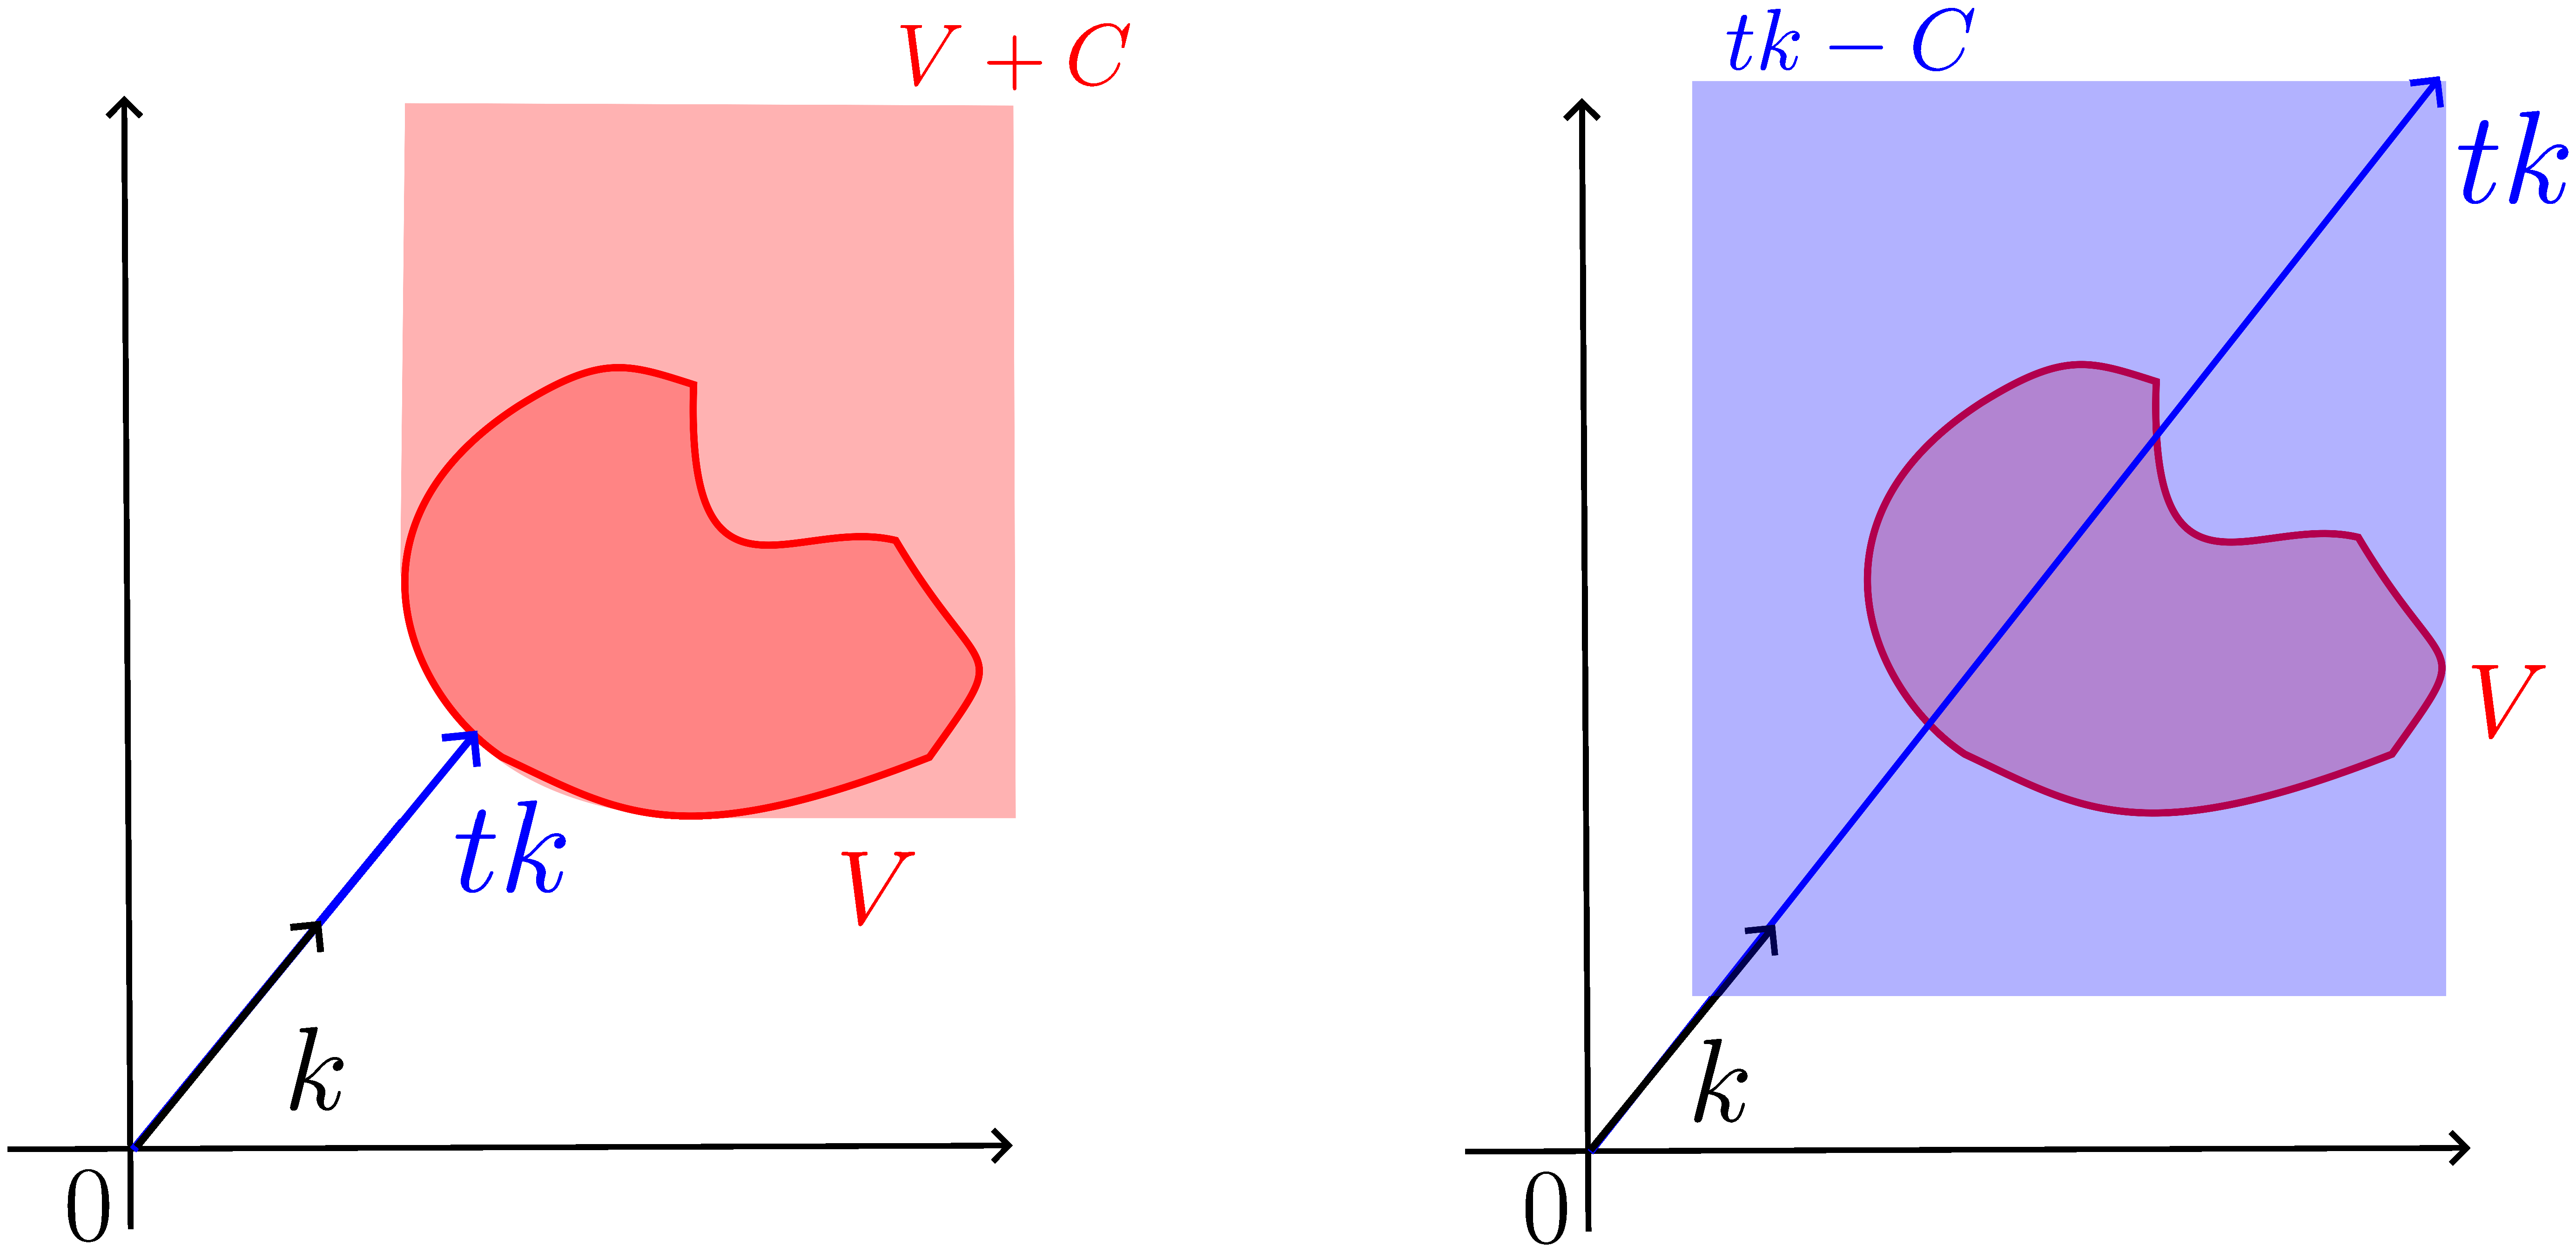
\includegraphics[keepaspectratio, scale=0.10]{figures/eps/tammar_scalarization_example.eps}
\end{frame}


\begin{frame}{Hiriart-Urruty Oriented Distance}
  \begin{block}{Definition (Hiriart-Urruty distance)}
    Let $Y$ be a real normed vector space. For a set $A \subset Y$, let the oriented distance function
    $\Delta_{A} \colon Y \to \RealNumberSet\cup\{\pm \infty\}$ be defined by
    \begin{align*}
      \Delta_{A}(y) \coloneq d_{A} (y) - d_{Y \backslash A}(y),
    \end{align*}
    $ d_{A} (y)= \inf\{\Norm{y - z} \mid z \in A\}$, $d_{\emptyset} (y) \coloneq + \infty$,
    and $\Norm{y}$ denotes the norm of $y$ in $Y$.
  \end{block}

  \begin{block}{Definition}
    For the set $A \in Y$, let the functions $\mathcal{D}^{+}_{A} \colon \mathcal{P}(Y) \to \RealNumberSet \cup \{\pm \infty\}$
    and $\mathcal{D}^{-}_{A} \colon \mathcal{P}(Y) \to \RealNumberSet \cup \{\pm \infty\}$ be defined as
    \begin{align*}
      \mathcal{D}^{+}_{A}(B) & \coloneq \sup\{\Delta_{A}(b) \mid b \in B\},\: B \in \mathcal{P}(Y),                            \\
      \mathcal{D}^{-}_{A}(B) & \coloneq \inf\{-\Delta_{A}(b) \mid b \in B\} = -\mathcal{D}^{+}_{A}(B),\: B \in \mathcal{P}(Y).
    \end{align*}
  \end{block}
\end{frame}

\begin{frame}{Hiriart-Urruty Oriented Distance}
  \begin{exampleblock}{Example}
    Let $Y = \RealNumberSet^{2}$, $A = [0,2] \times [0.2]$, $y_{1} = (1,1)$, and $y_{2} = (3, 3)$. Then,
    \begin{align*}
      \Delta_{A}(y_{1}) & = d_{A}(y_{1}) - d_{Y \backslash A}(y_{1}) = 0 - 1 = -1,        \\
      \Delta_{A}(y_{2}) & = d_{A}(y_{2}) - d_{Y \backslash A}(y_{2}) = 1 - 0 = \sqrt{2} .
    \end{align*}
  \end{exampleblock}
  \centering
  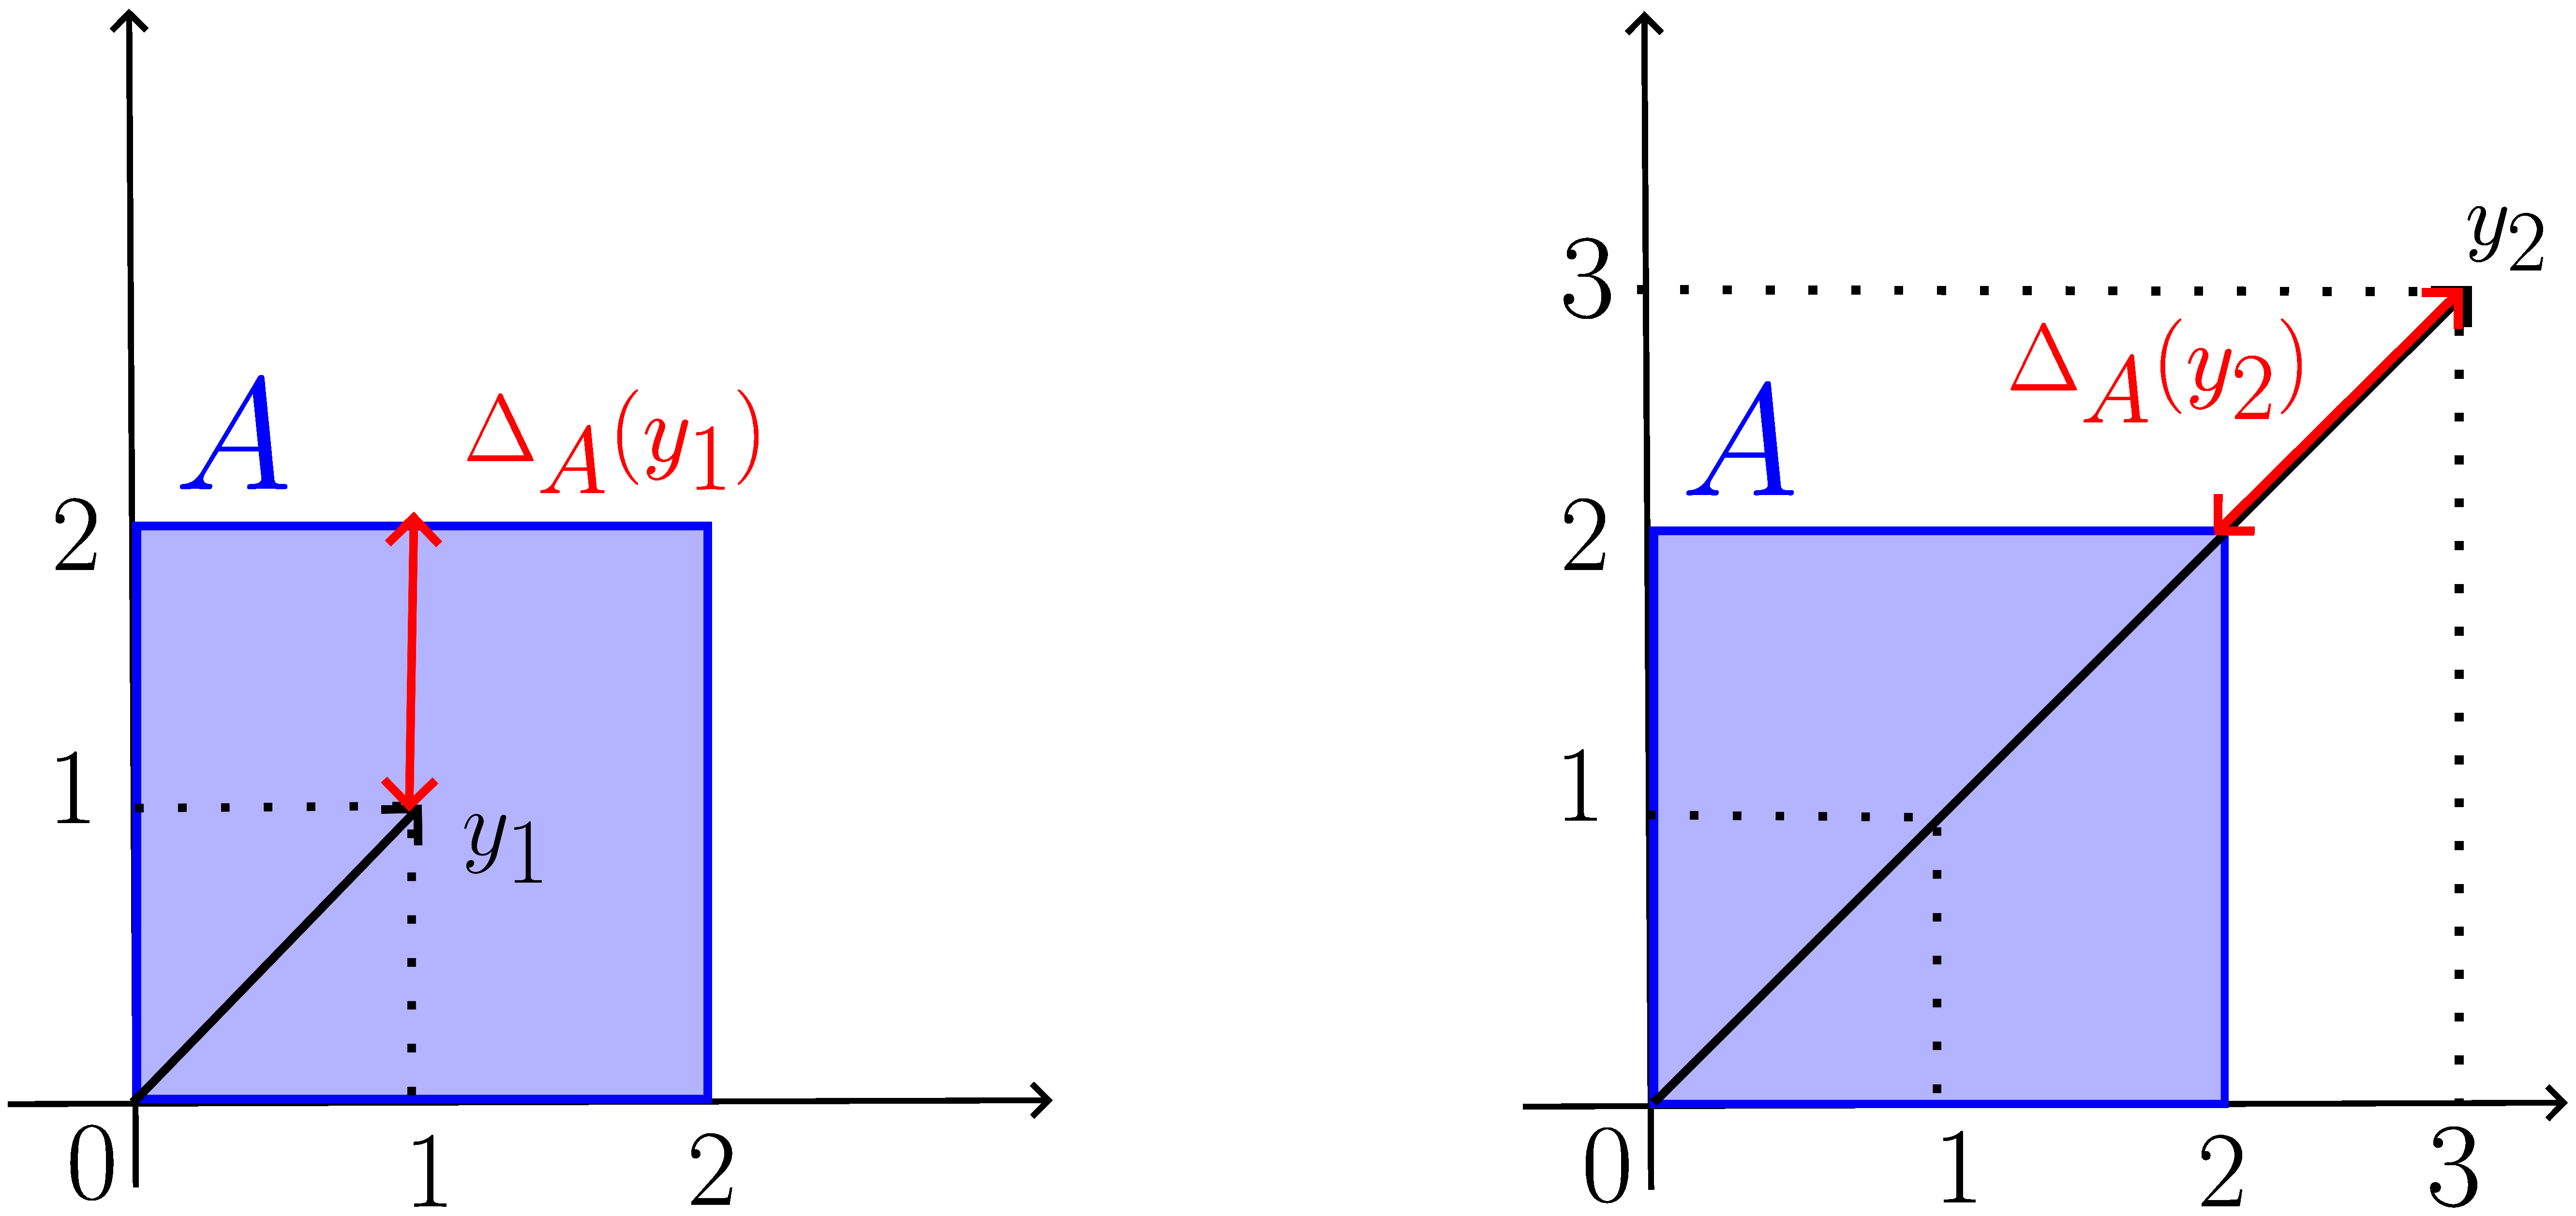
\includegraphics[keepaspectratio, scale=0.10]{figures/eps/hiriart-urruty_distance_example.eps}
\end{frame}

\begin{frame}{Applications}
  \begin{block}{Theorem}
    Let $X$ be a nonempty compact convex subset of a topological vector space,
    $Y$ a real normed vector space, $C$ a closed convex cone in $Y$ with $\Interior{C} \ne \emptyset$,
    and, $F\colon X \times X \to \mathcal{P}(Y) \backslash \{\emptyset\}$ a set-valued map.
    If $F$ satisfies the following conditions:
    \begin{enumerate}
      \item there exists $x_0, y_0 \in X$ such that $(\varphi \circ F)(x_0,y_0) \in \RealNumberSet$,
      \item for each fixed $y \in X$, $F(\cdot,y)$ is $(\preccurlyeq_{2}, C)$-continuous (that is, $C$-upper continuous),
      \item for each fixed $x \in X$, $F(x,\cdot)$ is $(\preccurlyeq_{C}^{(3L)})$-naturally quasi concave,
      \item for all $x \in X$, $F(x,x) \preccurlyeq_{C}^{(3L)} \{\theta_{Y}\}$,
    \end{enumerate}
    then there exists $\bar{x} \in X$ such that $ F(\bar{x},y) \preccurlyeq_{C}^{(3L)} \{\theta_{Y}\} $ for all $y \in X$.
  \end{block}
\end{frame}


% 6. Conclusions
% ----------------------------------------------------------------
\section{Conclusion}

% 6.1
\begin{frame}{Conclusion}
  \begin{itemize}
    \item We gave a new result of set-valued Fan-Takahashi inequalities via scalarization  .
    \item Kuwano's result which is introduced at first implies the only (3L) type minimax inequality.
          This results in the same type minimax inequality holds
          while the scalarization function is the oriented distance function.
    \item We need to check other scalarization functions to satisfy our assumption.
  \end{itemize}
\end{frame}

% References
% ----------------------------------------------------------------
\begin{frame}[allowframebreaks]
  \printbibliography
\end{frame}

\begin{frame}
  Thank you for your listening!
\end{frame}

\begin{frame}{Theme}

  Get the source of this theme and the demo presentation from

  \begin{center}\url{github.com/matze/mtheme}\end{center}

  The theme \emph{itself} is licensed under a
  \href{http://creativecommons.org/licenses/by-sa/4.0/}{Creative Commons
    Attribution-ShareAlike 4.0 International License}.

  \begin{center}\ccbysa\end{center}
\end{frame}

\end{document}
